% for english documents: uncomment the next line with \newcommand and comment the line after that
% for german documents: comment the next line with \newcommand and uncomment the line after that
% might need to compile twice for correct application of language change

\newcommand{\doclanguage}{\toggletrue{english}}  
%\newcommand{\doclanguage}{\togglefalse{english}} 

% change the following information
\newcommand{\docauthor}{Alexander Kulibaba}
\newcommand{\doctitle}{The importance of Augmented Reality in remote collaboration and the social effects it has on the user}
\newcommand{\matrikel}{422 406}
\newcommand{\supervisor}{Dipl.-Inform.~Hattori Hanzo }

\newcommand{\seminartitle}{Interaction in Virtual Worlds} %{Interaction in Virtual Worlds}
\newcommand{\seminartype}{Pro-Seminar} %{Pro-Seminar}
\newcommand{\term}{Summer Term 2022}
% if it is necessary to change more information on the titlepage take a look at titlepage.tex

%header for settings and package loading

\documentclass[
	a4paper, % A4 paper size
	12pt, %	larger font size
	BCOR = 1cm, % make inner margin (book) larger 
]{scrbook}
 
\usepackage{scrhack} % addition to koma script; disables warning concerning  \float@addtolists  in package listings
 
\usepackage{etoolbox} % for toggling options 
\newtoggle{english}
\doclanguage %execute the toggle for this

\iftoggle{english}
{
	\usepackage[english]{babel}
	\selectlanguage{english}
}
{
	\usepackage[ngerman]{babel}
	\selectlanguage{ngerman}
}

% Package for text and input type
\usepackage[T1]{fontenc}
\usepackage[utf8]{inputenc} %Linux: [utf8]; MAC: [macce]; Windows: [utf8]


\usepackage[absolute]{textpos} % for positioning logo

\setlength{\unitlength}{1mm} %one unit is equal 1mm
\tolerance = 9000 % avoid that text gets wider the textwith

\usepackage{
	graphicx, % include graphics
	varioref, % comfy references -> \label + \vref + \vpageref
	listings, % for listings
	enumerate,% for enumerations
	epstopdf, % convert eps figures to pdf
	multirow,  % for multirows and columns in tables
	longtable % for tables longer than one page
}


% better floats for floating around figures and tables
\usepackage{float}
\restylefloat{table}
\restylefloat{figure}

% define how captions should look like
\usepackage[bf,small]{caption}

\usepackage[hang,nooneline]{subfigure} % create subfigures with own captions

\usepackage{calc}

% line under chapter/section name
\usepackage{scrlayer-scrpage}
\pagestyle{scrheadings}
\setheadsepline{0.4pt}

\usepackage[nottoc]{tocbibind} %bibliography in table of content
\usepackage{babelbib} %References in the corresponding language
\bibliographystyle{gerapali} 

% avoid errors due to old font commands in gerapali
\DeclareOldFontCommand{\sc}{\normalfont\scshape}{\@nomath\sc}
\DeclareOldFontCommand{\em}{\normalfont\itshape}{\mathit}

% this package has to be included last!
\usepackage[
	pdftitle={\doctitle},
	pdfauthor={\docauthor},
	pdfpagemode=UseOutlines,
	colorlinks=true,
	linkcolor=black,
	urlcolor=black,
	citecolor=black,
	plainpages=false,
	hypertexnames=false,
	pdfpagelabels=true,
	hyperfootnotes=false,
	hyperindex=true 
	]{hyperref} 

 %definition of all packages etc.

\begin{document}
\iftoggle{english}
{
\newcommand{\submittedTo}{The present work was submitted to Visual Computing Institute}
\newcommand{\doctype}{Seminar Thesis in Computer Science by}
\newcommand{\matrikelWord}{Student ID Number:}
\newcommand{\supervisorWord}{Supervisor:}
}
{
\newcommand{\submittedTo}{Diese Arbeit wurde vorgelegt am Visual Computing Institute}
\newcommand{\doctype}{Seminararbeit im Studiengang Informatik von}
\newcommand{\matrikelWord}{Matrikelnummer:}
\newcommand{\supervisorWord}{Betreuer:}
}

\newcommand{\supervisorcontent}{Prof.~Dr.~Torsten W.~Kuhlen} 
\newcommand{\university}{Rheinisch-Westf\"alische Technische Hochschule Aachen}
\newcommand{\faculty}{Lehrstuhl f\"ur Informatik XII}
\newcommand{\institute}{Virtual Reality \& Immersive Visualization}


\begin{titlepage}
	
	\vspace*{-2cm}
	\makebox[\textwidth][l]{
		\hspace*{6cm}
		
\includegraphics[width=0.7\textwidth]{figures/rwth_vci_rgb.png}
	}
	
	\begin{center}
	\textbf{\submittedTo} \\
		
	\vspace{3cm}
	
	\begin{Large}	
		\seminartitle \\
		\seminartype{} \term \\
		\vspace{1cm}
		\doctitle \\
	\end{Large}	

	\vfill
	
	\doctype\\
	
	\vspace{0.5cm}

	\docauthor \\
	\matrikelWord{} \matrikel \\
	
	\vspace{2.5cm}
	
	\supervisorcontent \\ 
	\institute
	
	\vspace{0.5cm}

	\supervisorWord{} \supervisor \\

	\end{center}
	
\vspace{1cm}

\begin{flushright}
	Aachen, \today
\end{flushright}

\end{titlepage}

\cleardoublepage


\pagenumbering{roman}
\tableofcontents

%comment the follwoing line for first and final submission (only used for literature research)
%\chapter*{Literature List}
\addcontentsline{toc}{chapter}{Literature List}

Please remove this literature list after the \textit{Literature Research and Outline} deadline. 

% edit the following table for your literature list
\begin{longtable}{|p{5cm} | p{9cm}|}
	\hline
	\multicolumn{2}{|c|}{\textbf{Main Paper}} \\ \hline
	\cite{Hanzo2004} & State in a few sentences what the paper is about. \\ \hline
	\multicolumn{2}{|c|}{\textbf{Related Work}} \\ \hline
	\cite{Dam1998} & Excellent paper about quaternions. Presents slerp and squat quaternion interpolation. \\ \hline	
	 $\left[...\right]$ & Information on other interesting work... \\ \hline
	\multicolumn{2}{|c|}{\textbf{Focus 1}} \\ \hline
	\cite{Badler1994} & Great work about something. Badler writes always interesting things about this. \\ \hline
	  $\left[...\right]$& Some sentences about an even more interesting paper ... \\ \hline
	 $\left[...\right]$& Some sentences about an even more interesting paper ... \\ \hline
	\multicolumn{2}{|c|}{\textbf{Focus 2}} \\ \hline
	  $\left[...\right]$& Please replace \textbf{Focus 1}, ..., \textbf{Focus n} according to your topic.  \\  \hline
	  $\left[...\right]$& The longtable environment lets you extend your table over more than one page.\\ \hline
	  $\left[...\right]$& Some sentences about an even more interesting paper ... \\ \hline
 	\cite{Fowler2000} & Last example on this literature list. \\
	 \hline
\end{longtable}


\cleardoublepage
\pagenumbering{arabic}

% here you can include separate files for every section
\chapter{Introduction}
\label{sec::introduction}

Abstract:

Remote Working has gained a lot of importance last few years, primarily due to the pandemic forcing many employees out of their offices. This lead to many companies adapting to the new circumstances and transferring to remote work, and as the employees adapted as well, the upsides of remote working became very clear: no commute times, flexible working hours, and a big decrease in costs for office maintenance like cleaning and electricity, just to name a few. In short, it is a clear case that Remote Work is here to stay. However, everything has its downsides: Due to the heavy reliance on 2D video conferencing tools like Zoom, social interactions and meetings become drastically less efficient, because they cannot reproduce nonverbal behavior like eye contact or gestures, which makes these interactions less natural. This is where Augmented Reality (AR) comes in. With AR technology improving at very fast speeds, it has the potential to solve many problems that emerged with remote work, especially the social aspect. In this paper, I am going to explore how the design of a virtual avatar and its interaction with the real world impacts the social effects it has on the user.


\section{What is Augmented Reality?}

A topic that gathered more attention than any other in the current tech space is Augmented Reality or AR for short. In its most basic definition, this technology allows the user to project virtual objects onto the real-world 3d space and allows for interaction between real people and a virtual environment, that can contain everything from simple overlays to complex structures and virtual worlds. \cite{Carmigniani:2011te}

The time when Augmented Reality was just a fancy demo is long gone, it has been playing a big part in many people's everyday lives, and its influence is projected to only get bigger in the future. AR is built into many current technologies, from entertainment purposes like the captivating phenomenon that was the mobile game "Pokemon Go", where AR played a big part in the game’s rise to popularity, to useful everyday appliances like the heads-up displays that are built into many modern cars. AR is so useful in fact, that it is projected to be one of the fastest-growing industries in the next decade \cite{XR_Projection}. These were only some of the applications in the private sector, but currently, the biggest upsides for AR are in the industrial sector. Many big companies invested billions of dollars to develop the most cutting-edge AR technologies and to gain an early lead in their market. Just to name the biggest competitors, there is Microsoft with the HoloLens, Meta with their rendition of AR glasses, and Apple, which is rumored to develop an AR product of their own. It is safe to say that there is a lot of potential in augmented Reality when every single one of the biggest players in tech decides to make AR a priority in its development and invests billions in it. 

However, AR is not limited to a particular type of display technology nor only to visual overlays to the real world. AR can just as well be applied to all senses like smelling or hearing, but it is less popular in these forms and has not found many appliances yet. That is why in this paper the focus lies on the visual aspect of AR, especially on wearable AR headsets like the Microsoft Hololens, where the user wears a headset that computes the spacial position and rotation of the user's head by tracking the room with cameras and superimpose virtual content onto the real world by displaying it right in front of the user's eyes.

\section{The importance of Social Presence}
A pleasant user experience in a virtual environment depends on several factors, one of which is the perceived presence of the user, meaning that the user feels connected to the virtual environment and the interactions feel authentic and natural \cite{PresencePaper}. By introducing social interactions into the virtual environment, social presence becomes very important as well. The social presence of virtual characters plays a key role in how effective AR will be in replacing 2D video conferencing. It can be loosely defined as the sense of "being together" with another person through a virtual medium. It is important for social presence to be perceived as high because as many studies confirmed, a high social presence leads to greater satisfaction in the collaborators and improved quality in social interactions, which in turn leads to improved performance, which will be discussed further in the main part. In remote collaborations through AR, a collaborator's virtual embodiment is referred to as their avatar and the virtual embodiment of virtual characters are called virtual agents. The realism of these avatars and agents greatly influences the perceived social presence as well, and in the main part, we will discuss what the important variables in designing virtual characters are to maximize their perceived social presence. \cite{10.1117/12.387188}
Unlike in Virtual Reality (VR), where the user is fully immersed in a virtual world, AR adds a virtual overlay onto the real world, and studies show that this creates a high degree of social presence which makes it highly beneficial for remote collaboration.

\section{Why remote work is here to stay}

Even before covid, remote work was on the rise because many costs can be saved by working from home. Studies by Raffael Ferreira et al. found that remote work done right improves the work-life balance, and schedule flexibility of workers while greatly reducing costs for companies. Costs like travel expenses and catering can be saved and a cheaper workforce from other countries can be hired without complications. However, the study also finds that by working remotely many problems can occur: communication between workers suffers due to the collaborators not being able to read the body language and less visual contact in general \cite{joitmc7010070}. These problems can be addressed with the help of AR and technologies that will be shown in this paper.



\chapter{Related Work}
\label{sec::relatedwork}

There are already some papers that explore social aspects of AR, as well as how Avatar's appearance affects the social presence and how AR can be used for remote collaboration.

\section{The Effect of Avatar Appearance on Social Presence in an Augmented Reality Remote Collaboration}
\label{effectOfAvatarAppearance}

\begin{figure}[H]
\centering
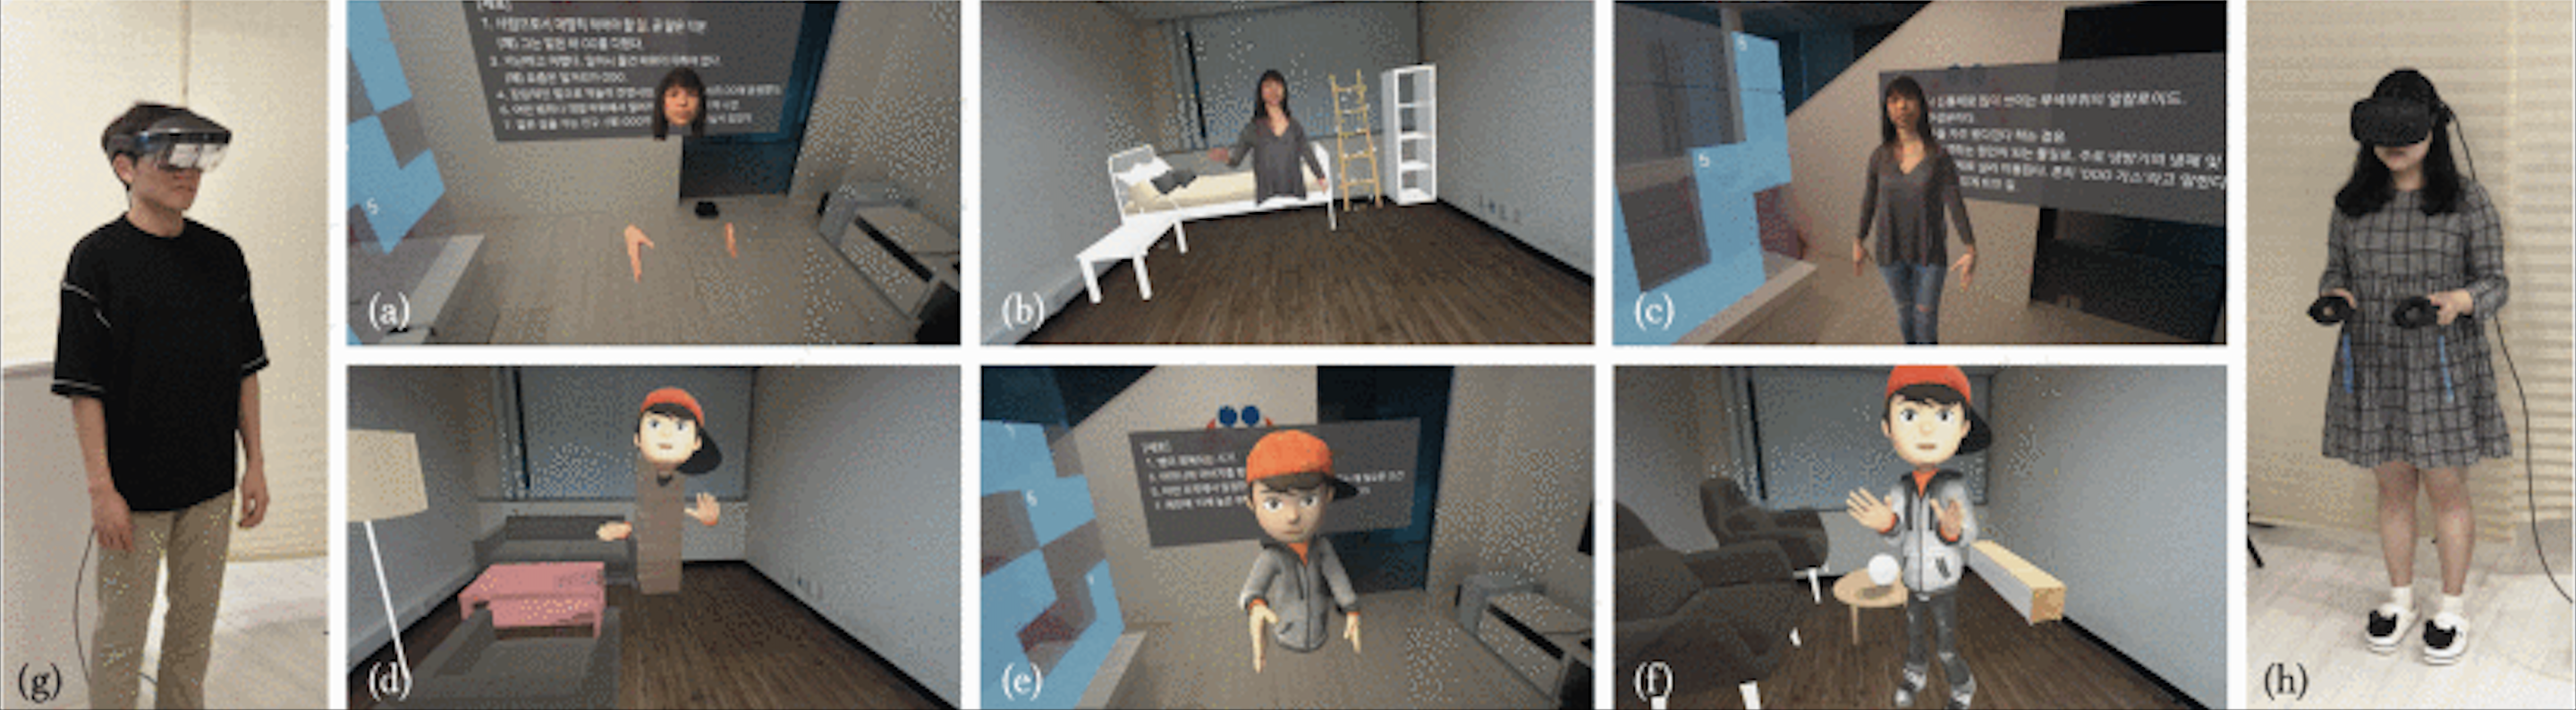
\includegraphics[width = 0.8\textwidth]{figures/Bildschirmfoto 2022-06-10 um 18.07.25}
\caption[Study 1 setup]{different avatar appearances}
\label{fig::avatarAppearences}
\end{figure}


The paper "The Effect of Avatar Appearance on Social Presence in an Augmented Reality Remote Collaboration" \cite{8797719}explores the effects some avatar design choices have on the user and how different visual representations of virtual agents will influence the social presence and user perception in an AR environment. To test this, a study was conducted, where 24 participants were asked to perform experimental tasks with an avatar, who was representing a remote collaborator, played by an actor. The avatar was displayed in one of six ways by changing the variables of Body part visibility and character style, which resulted in the following conditions: Realistic Whole Body (RWB), Realistic Upper Body (RUB), Realistic Head and Hands (RHH), Cartoon Whole Body (CWB), Cartoon Upper Body (CUB), Cartoon Head and Hands (CHH) as seen in Figure \ref{fig::avatarAppearences}.

\begin{figure}[H]
\centering
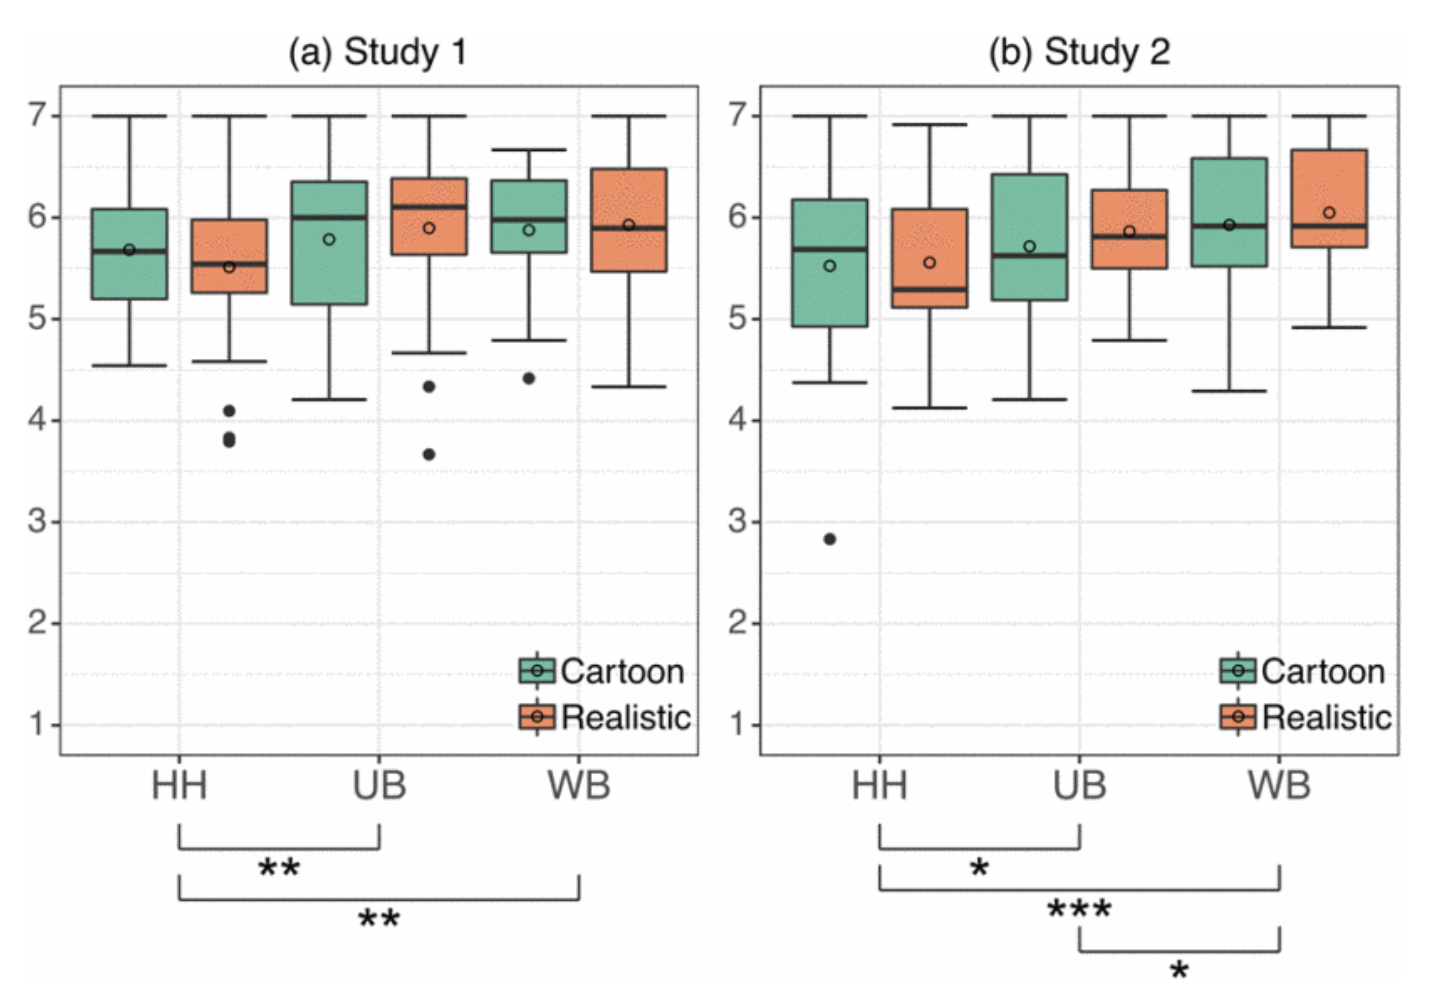
\includegraphics[width = 0.8\textwidth]{figures/Bildschirmfoto 2022-06-10 um 19.33.46}
\caption[Study 1 setup]{Aggregated social presence (1: Strongly disagree - 7: Strongly agree)}
\label{fig::avatarAppearences2}
\end{figure}


The study found that the Realistic Whole Body avatar was perceived as the most social present, with Cartoon Whole Body being a close second, and Head and Hands having the worst effect on the participants, both in cartoon and in realistic form as seen in \ref{fig::avatarAppearences2}.



\section{Social interaction in augmented reality}

The Paper “Social interaction in Augmented Reality” 
\cite{Carmigniani:2011te}
 focuses on the way augmented reality affects social interactions by creating three studies that mimick social situations with the addition of Augmented Reality, which infuses the situation with additional information. 

\subsection{Social inhibition and facilitation}
One interesting study was how the presence of virtual characters in the AR space influences people's task performance in the physical world. It is known that the presence of other people affects the task performance of humans, and it is a thoroughly studied theory in social psychology: social facilitation and inhibition. It refers to the fact that people tend to perform better in simple tasks when in the presence of other people, but on the other hand they perform worse on complex tasks. Zajonc’s drive theory can explain these tendencies: the presence of other people leads to an increase in one’s arousal, which in turn leads to better performance in simple tasks but a disadvantage in the execution of complex tasks.

\begin{figure}[H]
\centering
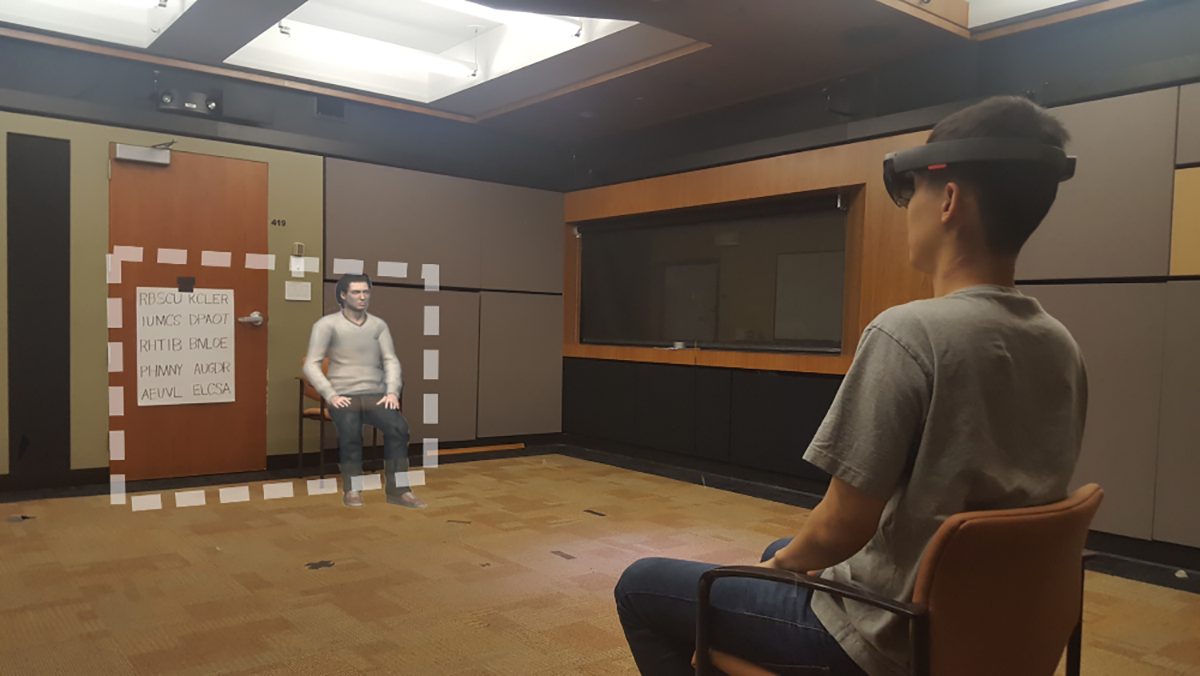
\includegraphics[width = 0.5\textwidth]{figures/pone.0216290.g001.PNG_L.png}
\caption[Study 1 setup]{This Figure shows the setup in which the study was conducted in}
\label{fig::firstSetup}
\end{figure}


This behavior has been tested and confirmed in Virtual Reality, but Miller’s paper focuses on these patterns in Augmented Reality. Due to the differences in surroundings and the presence of virtual characters instead of real humans, this behavior might be different in AR. To test this, they created a study recording the cognitive abilities of 60 participants by having them solve anagram tasks under the following conditions: Each participant was sitting alone in a 5.6 m by 6.4 m room equipped with a Microsoft HoloLens headset. A virtual agent would introduce himself, and the participant was informed that the agent would either stay during the completion of the task or leave the room, depending on the conditions, as shown in \ref{fig::firstSetup}. After that, the participants had three minutes to solve as many anagrams as they could, which were either hard or easy to solve, and read their answers out loud as soon as they solved them. This process was executed four times per participant, one time per combination of difficulty and social context. 


\begin{figure}[H]
\centering
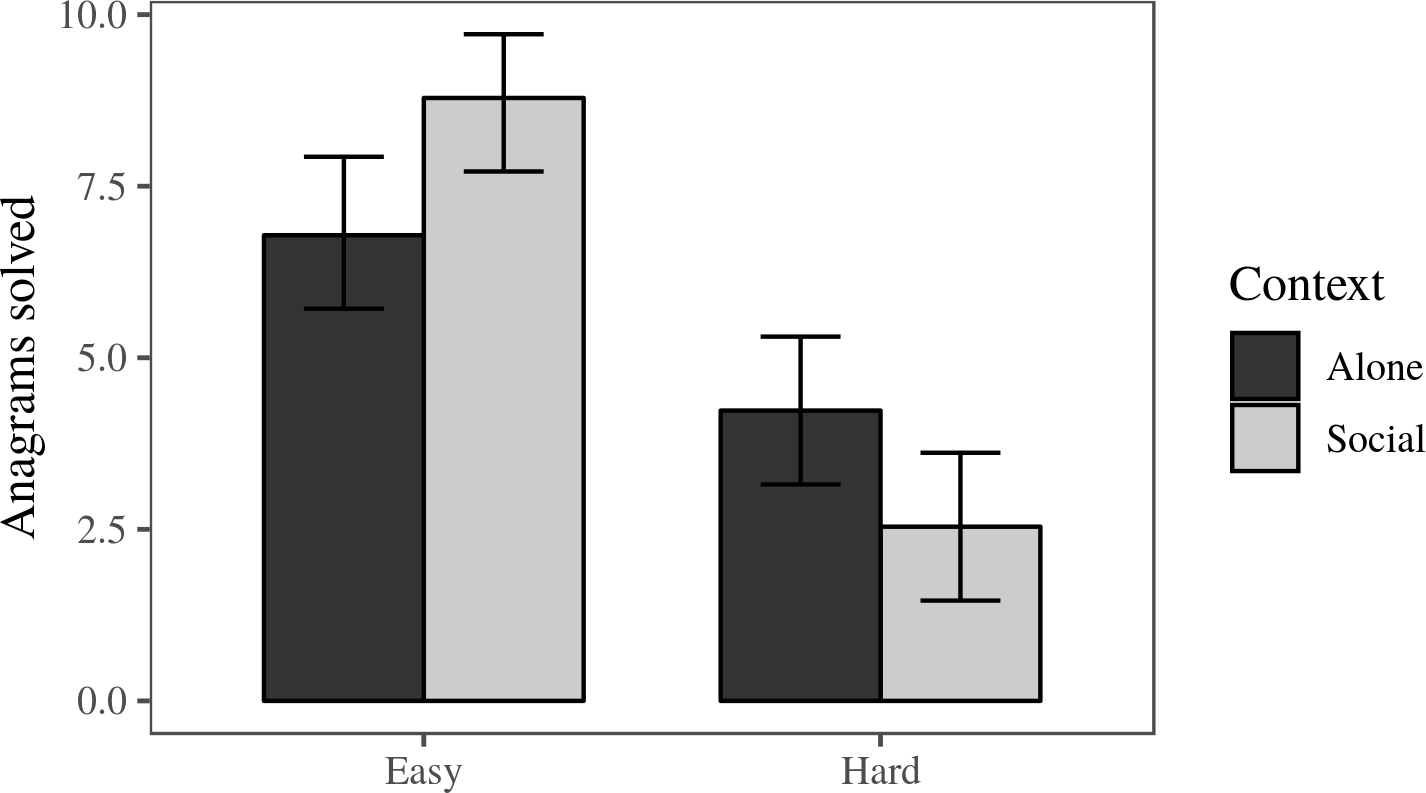
\includegraphics[width = 0.5\textwidth]{figures/pone.0216290.g003.PNG_L.png}
\caption[Study 1 result]{Results of the first study}
\label{fig::firstResult}
\end{figure}


Results showed that, like their physical counterparts, virtual agents indeed influence the performance of the participants as shown in \ref{fig::firstResult}. The participants performed significantly better at easy tasks with a virtual agent present while performing worse at harder tasks. With these results, it is clear that social facilitation and inhibition both exist even in Augmented reality with virtual agents.


One very interesting observation was how the participants improved their performance at the given tasks over time and how the effects of social facilitation and inhibition did not extend over multiple trials. This can be an indicator that the realism of the virtual agent is not high enough and that the participants get accustomed to the presence of the agent which in turn lowers the social pressure.

\subsection{Social norms in AR}

\begin{figure}[H]
\centering
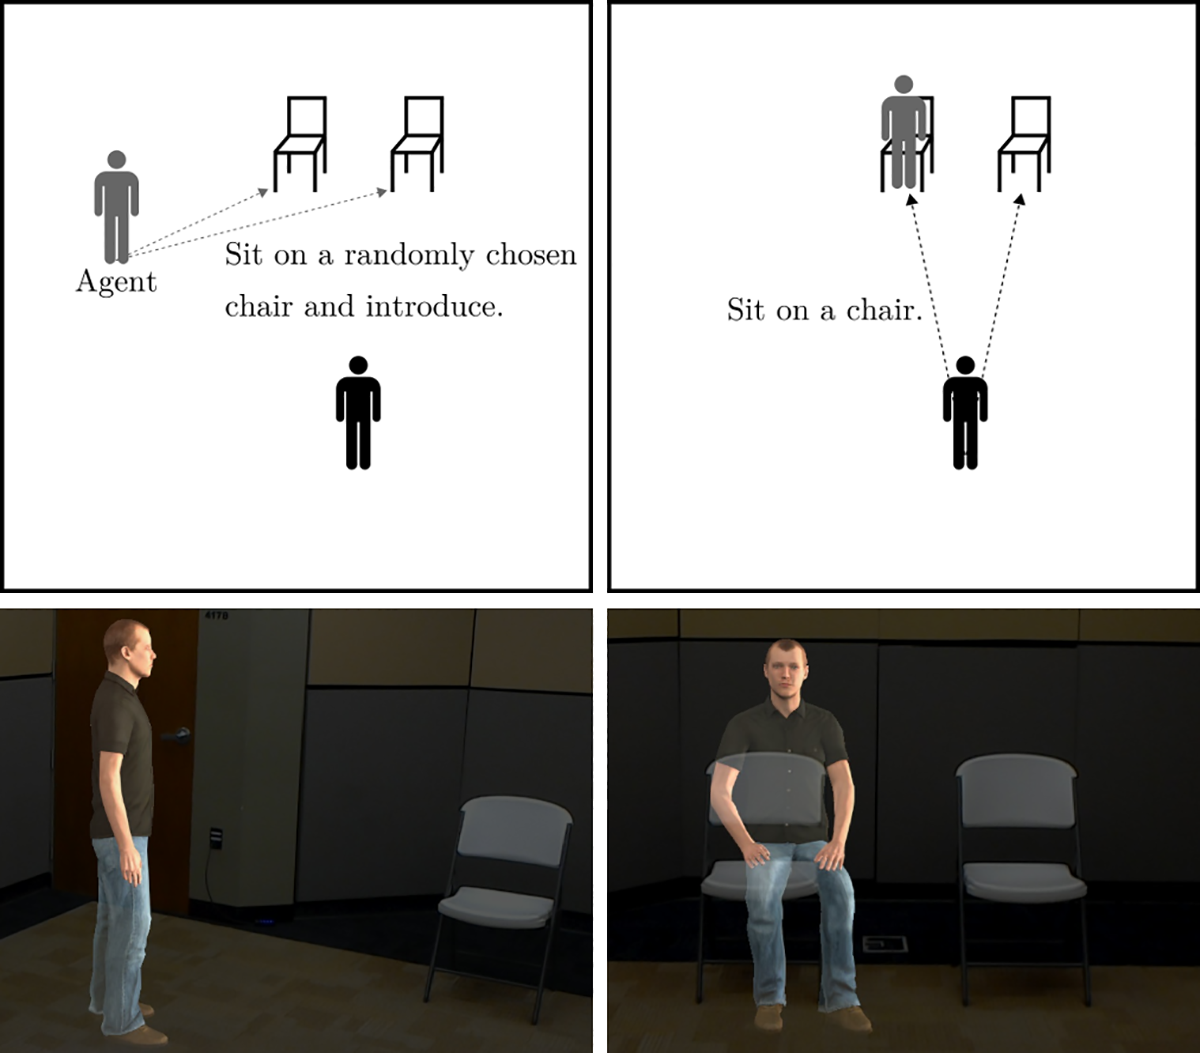
\includegraphics[width = 0.5\textwidth]{figures/pone.0216290.g004.PNG_L.png}
\caption[Study 1 result]{Setup of the second study}
\label{fig::secondStudy}
\end{figure}

In the second study of the paper, they tested if participants would adapt their nonverbal behavior including interpersonal distance and eye contact in the presence of a virtual agent. Additionally, they tested if the effect lasts even after taking the headset off. The procedure was the following: The participants were randomly assigned one of two conditions, either "Headset" or "without Headset". Under both conditions, the participants started with a headset and saw a virtual agent walk across the room and sit down in one of two chairs as shown in \ref{fig::secondStudy}. After that, only the participants with the "without Headset" conditions took off their Headset and the participant was asked to sit on one of the two chairs. 

After conducting the study, it was clear that the participants wearing the Headset avoided sitting on the agent, and the participants without the headset were still significantly more likely to sit on the chair without the agent, even without seeing him.
\subsection{Social connectedness between AR users and non-users}

The goal of the last study of the paper was to test if the social connectedness between people suffers if one person is wearing an AR headset. To test this, two random participants were put in a small room, with one participant wearing an AR headset and the other one not. There were two possible conditions: in the virtually occluded condition, there was a logo superimposed onto the other participant, in the not virtually occluded condition the logo was next to the partner. Then, the participants were asked to discuss something interesting that happened to them in the past month for 5 minutes, and afterward, they both completed a questionnaire about the experience where they ranked their social connectedness from 1 to 5.

The results showed that there was no significant difference in the social connectedness, interpersonal attraction, and social presence between virtually occluded and not virtually occluded users. However, regardless of condition, AR users tend to have a lower social presence, connectedness, and interpersonal attraction than the person not using the headset.

\section{Collaborative Augmented Reality}

This paper explores the collaborative aspect of AR and how it can be used to improve face-to-face and remote collaboration \cite{CollaborativeAR}. AR offers many benefits, like seamless interaction between real and virtual environments and the ability to enhance reality, which is really useful when collaborating. In this paper, collaboration gets split into two categories: remote collaboration and face-to-face collaboration. in both cases, AR offers many benefits.

\subsection{face-to-face collaboration}
For face-to-face collaboration, when discussing virtual objects, many non-verbal cues get lost. For example, discussing an object on the screen can be frustrating because there is no way to reference on-screen objects with the precision and intuition of real objects. Augmented Reality can be used to project onto and enhance the physical workspace for face-to-face collaboration and improve the efficiency of these kinds of collaborations by making them very intuitive, even when rendering 3D models.

\begin{figure}[H]
\centering
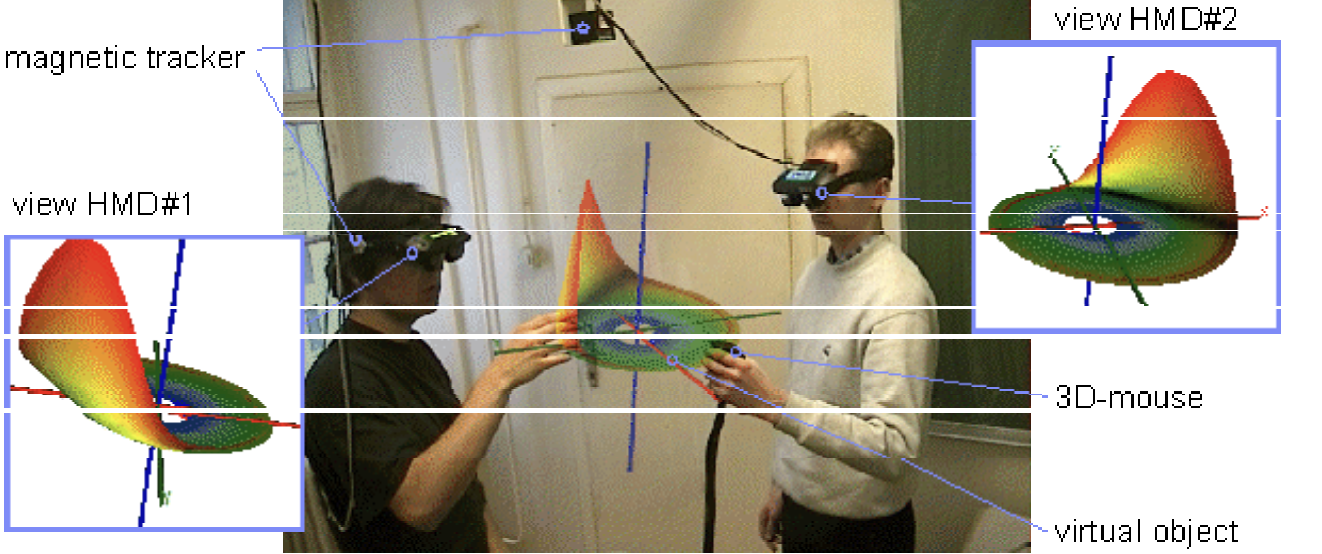
\includegraphics[width = 0.5\textwidth]{figures/Bildschirmfoto 2022-06-10 um 18.47.26}
\caption[Study 1 setup]{This Figure shows the StudierStube AR interface}
\label{fig::StudierStube}
\end{figure}

 A study at StudierTube by Schmalsteig et. al. \cite{studierstube} tried out face-to-face collaborations by having two participants wear see-through head-mounted displays and collaboratively view a 3d-object superimposed onto the real environment. By reporting this process they found these main benefits for collaborative AR environments:

\begin{itemize}
\item Virtuality: Objects that don’t exist in the real world can be viewed and examined. 
\item  Augmentation: Real objects can be augmented by virtual annotations. 
\item  Cooperation: Multiple users can see each other and cooperate in a natural way. 
\item Independence: Each user controls his own independent viewpoint.
\item Individuality: Displayed data can be different for each viewer.
\end{itemize}

Additional studies by Billinghurst et al. explored the benefits of AR collaboration by comparing the approach to problem-solving in face-to-face collaborations with real objects, co-located AR collaboration with virtual objects, and co-located projection screen-based collaboration with virtual objects. The results showed that speech and gesture behaviors in face-to-face and AR problem solving were very similar, which underlines the improved intuition with AR collaboration. However, the participants still felt that face-to-face conditions and AR were not similar, which can be attributed to the use of relatively old technology from 2002, so there is room for additional studies that test this with newer equipment.

\subsection{Remote collaboration}

In remote collaboration, AR has many applications as well. A user study by Billinghurst et al. found that AR video conferencing gave the participants a "significantly higher sense of presence" and that made it easier for participants to pick up on non-verbal cues, which are very important for high social presence. This paper, even while being from the Year 2002 when the AR technology was still very limited, saw big potential in AR remote conferencing.

\chapter{The possibilities of AR in remote collaboration }
\label{secMainPart}
\section{The possibilities of AR in remote collaboration}
The current standard for remote video conferencing are tools like Zoom, where all participants get recorded by a webcam and a microphone, and they communicate only through these mediums. This approach comes with many downsides. Firstly, the social presence with 2d video conferencing is very low, which leads to many problems. From an efficiency standpoint, higher social presence leads to improved task performance and time efficiency as discussed in the paper "Social interaction in augmented reality" \cite{10.1371/journal.pone.0216290} due to social facilitation. This means that with lower social presence from other participants, workers tend to perform worse and will not be as productive. Secondly, with increased social presence comes better working morale from the participants, because with many workers switching to home office came a greater feeling of social isolation \cite{joitmc7010070}. 
This impacts the workers' mental health negatively and worsens their performance and well-being. Again, by implementing AR into remote collaboration, the social presence will be improved and these problems will be solved. Through AR the social presence is increased, because it allows for Three-dimensional video conferencing which, as Hauber et al. found, increases social presence significantly \cite{2dSocialPresence}. Another study by Doherty-Sneddon et Al. \cite{taskPerformance} found that task efficiency 2d video communication is worse than face-to-face, meaning that it takes more words to transmit information in video communication than in face-to-face communication. This is mostly due to the fact that the visual signals it provided didn't help listeners understand in the same way as visual signals in face-to-face interaction did. Another important nonverbal cue that is missing in 2d-video-communication is eye-contact. Although eye contact is not necessary for the task to be completed successfully, it may have a significant impact on how satisfying the communicative experience is for users. This, again, leads to a reduction in efficiency and productivity of workers, while increasing the feeling of isolation because eye contact leads to greater sympathy between two collaborators.
\begin{figure}[H]
\centering
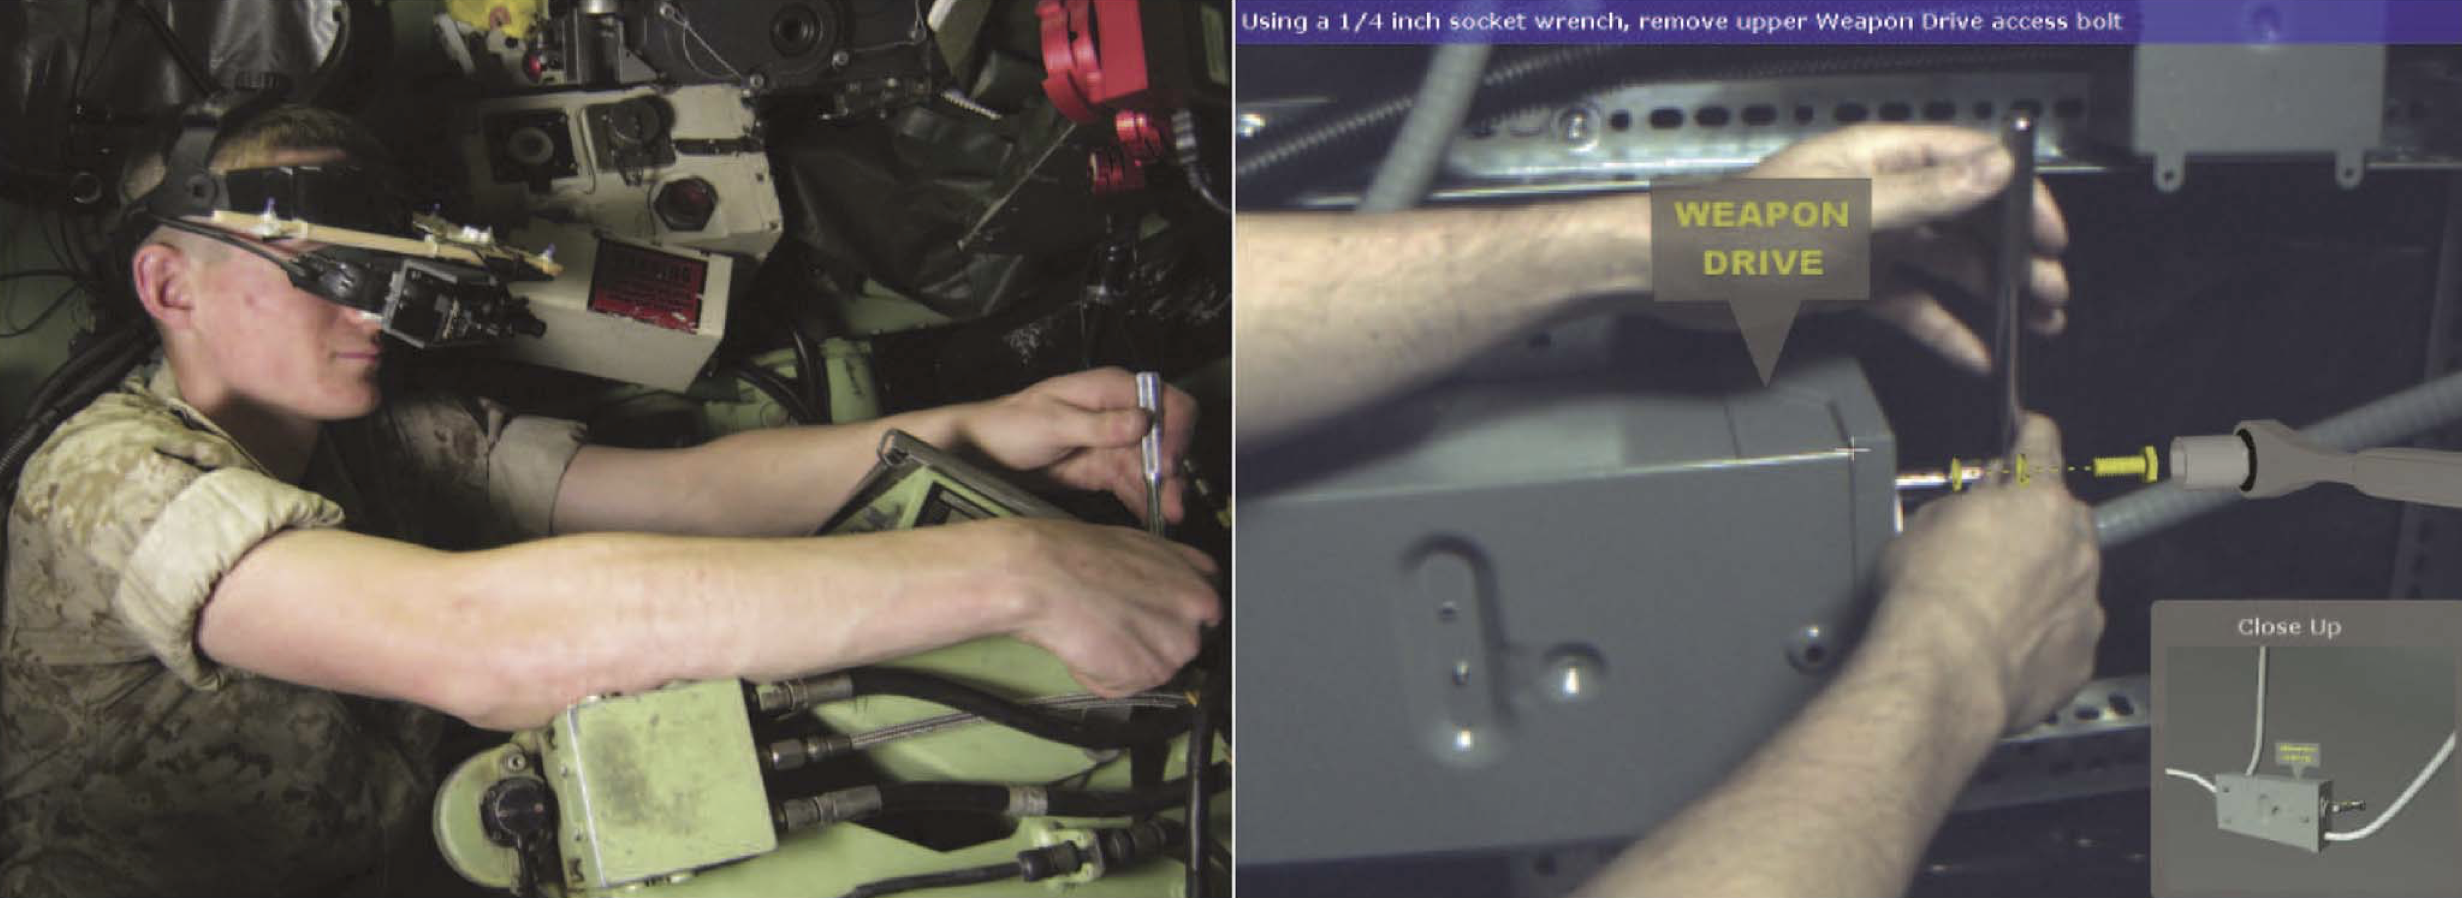
\includegraphics[width = 0.8\textwidth]{figures/ARmaintenance}
\caption[test]{(Left) A mechanic wearing a tracked headworn display removes a bolt from a component inside an armored personnel carrier turret. (Right) A view through the AR display virtually superimposing information onto the real world}
\label{fig::maintenance}
\end{figure}

Furthermore, when working on real-world problems like maintenance where fast problem-solving is required if some problem occurs, expert opinions play an important role. Because these problems have to be solved in the real world, they often cannot show up in person and have to collaborate remotely through video conferencing. This can lead to dramatically less efficient communication when trying to solve this problem remotely, because, as Billinghurst et al. concluded in their study, discussing real-world objects through 2D video conferencing is inefficient because non-verbal communication like pointing is crucial for intuitive collaboration \cite{CollaborativeAR}. AR offers the possibility of having a remote collaborator, represented by a virtual agent, projected onto the real world. This allows for remote collaboration that feels to both users like intuitive face-to-face collaboration and allows for more efficient workflows. Furthermore, information regarding the real-world objects can be superimposed onto them using AR as seen in \ref{fig::maintenance}, which makes the process much better because it enhances the efficiency of maintenance, especially with complex parts \cite{5620905}.

\section{Optimal Avatar design}
An important choice to make is the avatar design, because it greatly affects the perceived social presence of the avatar for the user as discussed in \ref{effectOfAvatarAppearance}. However, the optimal design choices for the avatar's appearance differ between distinct use cases, which makes it important to explore how different design choices affect the users' perception of the avatar.

The first important decision is the appearance of the Avatar. depending on the use case, different appearances can have different effects on the user. In general, it can be said that the more realistic the avatar, the better the interaction and the social connectedness. Latoschik et al. \cite{avatarRealism} found that a more realistic avatar finds better acceptance in users which leads to a better connectedness in collaboration. However, under certain circumstances, the study found that participants experienced an uncanny valley effect where if the avatar imperfectly resembles a realistic human being, the observers experienced a feeling of uneasiness and revulsion \cite{8797719}. 

\begin{figure}[H]
\centering
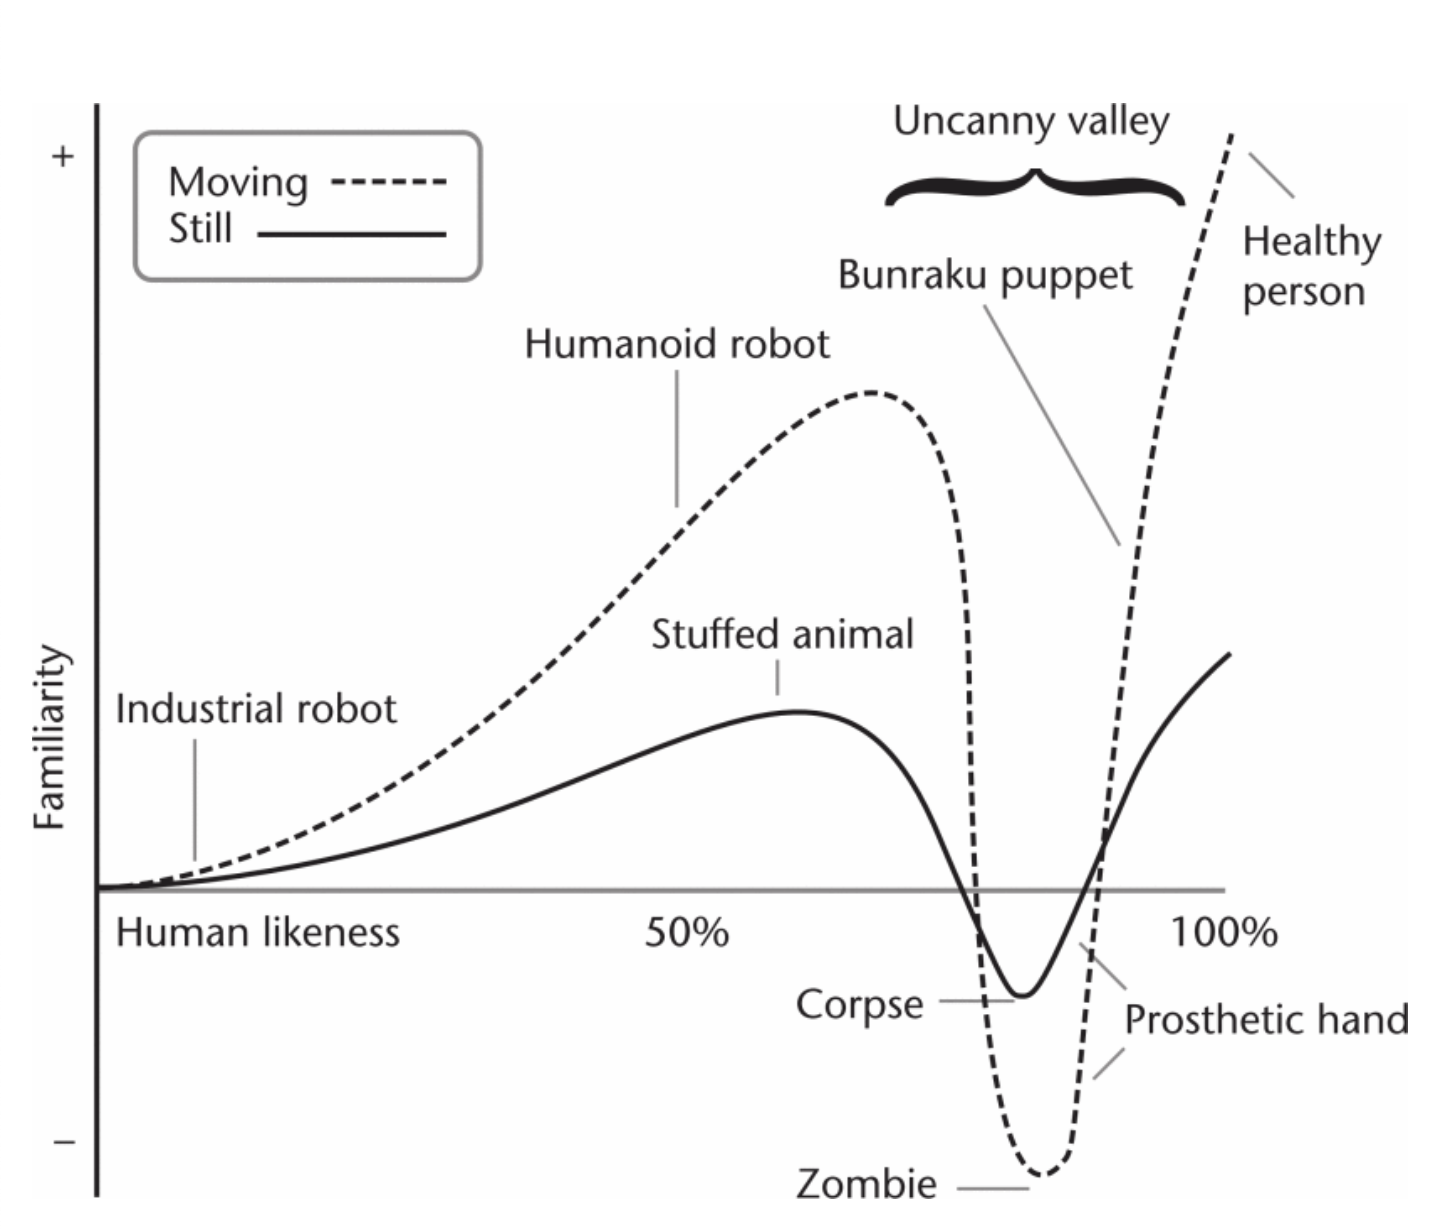
\includegraphics[width = 0.5\textwidth]{figures/uncannyValley}
\caption[Study 1 setup]{Visual representation of the uncanny valley effect}
\label{fig::uncannyValley}
\end{figure}

The uncanny valley effect is a controversial phenomenon that occurs when human or humanlike characters fail to arouse our sympathy and rather cause discomfort in the observer, even if it resembles a human closely. This means that when virtual characters approach realistic similarity to humans while still having imperfections, they become eerie or frightening. But when these similarities are perfected, the characters suddenly become very familiar again as seen in \ref{fig::uncannyValley}. \cite{4557950}

Due to these effects, it is important to take the computing power of the device in use into consideration: when rendering a realistic avatar, even small imperfections lead to great discomfort and uneasiness in users. This shows further research potential in this field, because with improved graphics the appearance of the avatar can be improved to better resemble realistic humans, which opens the possibility of overcoming the uncanny valley effect and having a greater distinction between cartoon and realistic avatars.

As Yoon et al. found in their studies, social Presence was highest with avatars that were realistic and where the whole body was visible, although, as already discussed, it resulted in an uncanny feeling in some participants. In general, Whole-body avatars were perceived as the most present, with avatars consisting of only the upper body getting positive recognition as well \cite{8797719}. This means that for remote collaboration, the avatar or virtual agent should at least be consisting of an upper body to feel natural to the user. 

\begin{figure}[H]
\centering
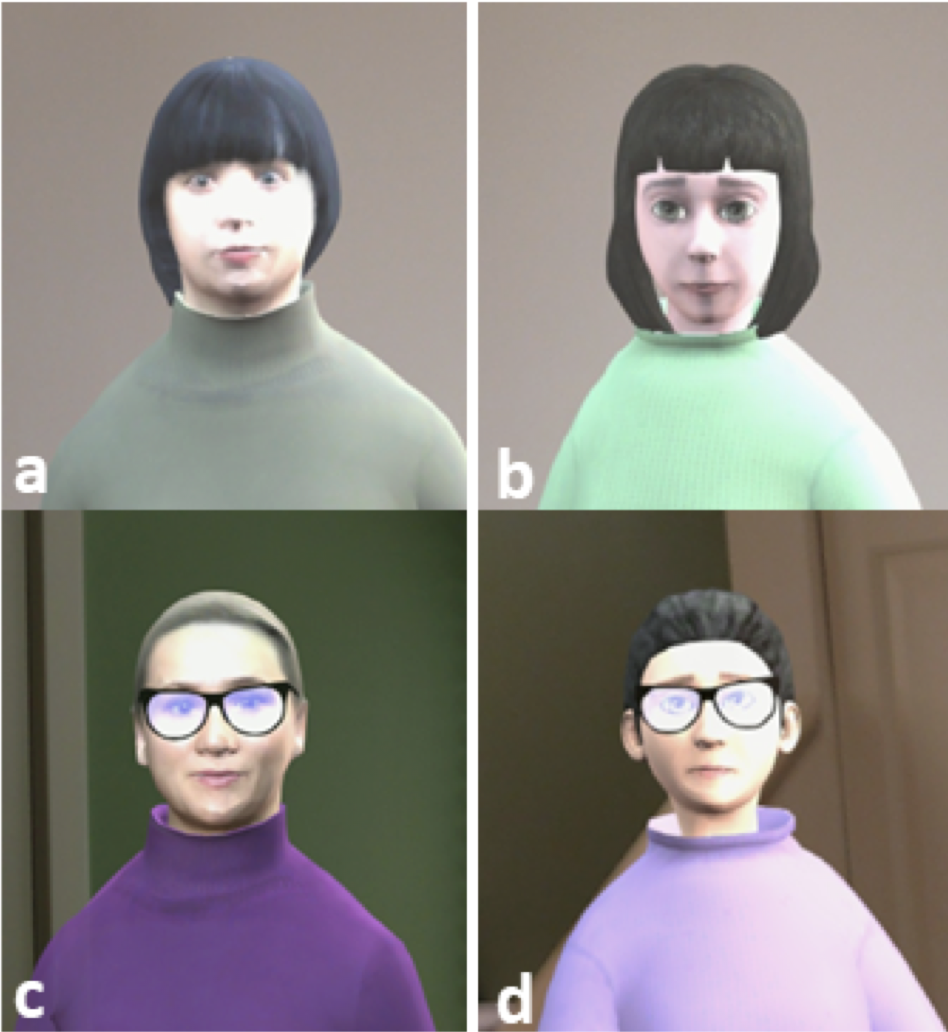
\includegraphics[width = 0.5\textwidth]{figures/Bildschirmfoto 2022-06-10 um 19.48.36}
\caption[Study 1 setup]{Example of realistic (a,c) and cartoon (b,d) avatar upper bodies}
\label{fig::solutions}
\end{figure}

Other studies at Microsoft from C. Dobre et al. \cite{Microsoft} concluded as well that a realistic appearance has better perceived nonverbal behavior and felt more appropriate to the participants than a cartoon avatar. This is especially interesting because the study was conducted in a working space, so it underlined the previous statements about their usefulness in work meetings. However, the study also found that the appearance of avatars got less important with time, meaning that the participants got accustomed to the avatars' appearance, no matter if realistic or cartoonish. Further work could elaborate on this study and test the reaction of younger participants to cartoon or realistic avatars. This way the perceived friendliness can be differentiated by testing different age groups and the most appropriate avatars for applications at schools or nursing homes can be found. Additionally, with improving technology it may be possible to improve the realism of the realistic avatars and remodel the cartoon avatars to be more appealing to children.

This does not mean however that cartoon characters do not have applications, because in general, while the realistic avatar was perceived as best for efficient collaboration and social presence, the cartoon characters gave the participants a sense of comfort and friendliness, as well as having the benefit of no uncanny valley \cite{8797719}. This means that realistic whole-body avatars are the best for collaborative environments, but cartoon whole-body or upper-body avatars are suited better for applications involving children or in general outside of the working environment.

\chapter{Conclusion}
We can conclude that remote working is as important as ever and Augmented reality has the potential to solve many problems that come with remote collaboration. A very important aspect is the design of the virtual avatar because the perceived social presence of virtual agents and avatars contributes significantly to the user having a pleasant experience.
Future work could improve on the studies and test the effect of different AR avatar appearances with varying groups of age or in different settings like in a hospital or school, not just work, because we found that different avatar appearances suit different needs, certain appearances are for example more professional while others are more friendly.

In general, this is definitely a topic to follow closely in the future because with the improvement of AR technology and additional investments from big tech companies the potential for solving these problems only grows.
\bibliography{literature}

\end{document}

